\section{Vectores aleatorios}

\subsection{Introducción}

\lb{Objetivo: }estudiar $k$ variables sobre una población de individuos (objetos).

\lb{Algunos ejemplos:}
\begin{itemize}[label=$\to$]
\item Las variables meteorológicas como temperatura, humedad y velocidad del viento.
\item La intensidad y la fase de una señal aleatoria que se miden en los canales de comunicación.
\item Los parámetros clínicos de los pacientes (como presión arterial, niveles de glucosa, etc.)
\end{itemize}
Habitualmente estas variables cualitativas o discretas que nos indicarán grupos de individuos.

Estas variables se representarán mediante vectores aleatorios sobre un espacio de probabilidad.

\begin{enumerate}[label=\arabic*)]
	\item Definiciones
\end{enumerate}

Un \lb{vector aleatorio} (v.a.) $k$-dimensional sobre un espacio de probabilidad $(\Omega,\mathcal{S},\mathcal{P})$ es $X=(X_1,\dots,X_k)$ tal que \[ X_i^{-1}(-\infty,x]\in\mathcal{S} \]para todo $x\in\R,\, i=1,\dots,k$

\begin{itemize}[label=\color{red}\textbullet, leftmargin=*]
	\item \color{lightblue}Función de distribución conjunta
\end{itemize}

$F:\R^k\longrightarrow[0,1],$\[ F(x_1,\dots,x_k)\coloneq P[X_1\le x_1,X_2\le x_2,\dots,X_k\le x_k], \] para todo $x_1,\dots,x_k\in\R$.

\subsection{Independencia de las variables aleatorias}

\begin{itemize}[label=\color{red}\textbullet, leftmargin=*]
	\item \color{lightblue}Definición
\end{itemize}
Las variables aleatorias $X_1,\dots,X_k$ son \lb{independientes} si los sucesos \[ \{x_1\le x_1\},\{X_2\le x_2\},\dots,\{X_k\le x_k\} \]son independientes para todo $x_1,\dots,x_k\in\R$.

Esto es equivalente a que \[ F(x_1,\dots,x_k)=P[X_1\le x_1]\cdot P[X_2\le x_2]\cdots P[X_k\le x_k] \]para todo $x_1,\dots,x_k\in\R$.


\subsection{Distribuciones marginales}

La función $F_{X_i}(x_i)=P[X_i\le x_i]$ se denomina \lb{función de distribución marginal} $i$-ésima y corresponde con la función de distribución de la variable aleatoria $X_i$

Las \lb{distribuciones marginales} pueden obtenerse a partir de la distribución conjunta: \[ F_{X_i}(x_I)=F(+\infty,\dots,+\infty,x_i,+\infty,\dots,+\infty) \]
Análogamente, la \lb{función de distribución marginal del subvector aleatorio} $(X_{i_1},\dots,X_{i_m})$ vendrá dada por \[ F_{X_{i_1},\dots,X_{i_m}}(x_{i_1},\dots,x_{i_m})=F(+\infty,\dots,+\infty,x_{i_1},+\infty,\dots,+\infty,x_{i_m},+\infty,\dots,+\infty). \]

\subsection{Vector aleatorio absolutamente continuo}

Un \vea $X$ es \lb{absolutamente continuo} si existe una función $f:\R^k\longrightarrow\R$ no negativa (llamada \lb{función de densidad}) tal que \[ F(x)=F(x_1,\dots,x_k)=\int_{-\infty}^{x_1}\cdots\int_{-\infty}^{x_k}f(z_1,\dots,z_k)\mathrm{d}z_k,\dots,\mathrm{d}z_1, \]para todo $x=(x_1,\dots,x_k)\in\R^k$

Usando el \lb{teorema fundamental del cálculo}, se tiene que en cada punto de continuidad $(x_1,\dots,x_k)$ de $f$: \[ \dfrac{\partial^kF(x_1,\dots,x_k)}{\partial x_1,\dots,\partial x_k}=f(x_1,\dots,x_k).\]

\begin{tikzpicture}
	\node[red, draw=red, fill=red!10, line width=1.5, text width=\textwidth] {Existen \vas cuya función de distribución es continua pero que no son absolutamente continuas (tienen una parte singular) y puede ocurrir que $X_1,\dots,X_k$ sean absolutamente continuas y que $(X_1,\dots,X_k)$ no lo sea.
	\begin{itemize}[label=$\to$]
	\item Ejemplo: Si $X_1$ es una \va absolutamente continua, entonces el \vea $X=(X_1,X_2)$ es continuo pero no absolutamente continuo.
	
	\item De hecho, es completamente singular ya que está contenido en la recta $y=x$ que tiene medida cero en $\R^2$.
	\end{itemize}
	Esto ocurre si consideramos las notas de unos alumnos y sus medidas. En estos casos deberemos eliminar estas variables dependientes del vector.
	};
\end{tikzpicture}

\subsection{Vector aleatorio discreto}
Un vector aleatorio $X$ se dice que es \lb{discreto} si existe un conjunto numerable $\mathcal{S}\in\R^k$ tal que $P(X\in\mathcal{S})=1$.

\lb{Función masa de probabilidad} de una vector aleatorio discreto: \[ P[X=x]=P[X_1=x_1,\dots,X_k=x_k] \]para todo $x=(x_1,\dots,x_k)\in\R^k$, satisfaciendo:
\begin{itemize}[label=$\to$]
\item $P[X=x]\ge0,\;\forall x\in\mathcal{S}$
\item $\sum_{x\in\mathcal{S}}P[X=x]=1$
\end{itemize}
\lb{Función de distribución} de un \vea discreto: \[ F(x)=P[X\le x]=\sum_{\begin{subarray}{c}
z\in\mathcal{S}\\
z\le x
\end{subarray}}P[X=z], \]para todo $x\in\R^k$.

\subsection{Distribuciones marginales}
\subsubsection{Caso continuo}
\begin{itemize}[label=\color{red}\textbullet, leftmargin=*]
	\item \color{lightblue}Distribución marginal de la variable aleatoria $X_i$
\end{itemize}
Sea $X=(X_1,\dots,X_k)$ un \vea continuo con función de densidad $f$ entonces cada componente $X_i$ es de tipo continuo y su función de distribución es; \[ F_{X_i}(x_i)=P[X_i\le x_i]=\int_{-\infty}^{x_i}f_{X_i}(z_i)\mathrm{d}z_i, \]con\[ f_{X_i}=\int_{-\infty}^{+\infty}\cdots\int_{-\infty}^{+\infty}f(z_1,\dots,z_k)\mathrm{d}z_1,\dots,\mathrm{d}z_{i-1}\cdot\mathrm{d}z_{i+1}\dots,\mathrm{d}z_k, \]para todo $z_i\in\R$.

La función de densidad marginal de cualquier subvector se calcularía de igual forma.

$X_1,\dots,X_k$ son \lb{independientes} $\longleftrightarrow f(x_1,\dots,x_k)=f_{X_1}(x_1)\cdots f_{X_k}(x_k)$.

\subsubsection{Caso discreto}
\begin{itemize}[label=\color{red}\textbullet, leftmargin=*]
	\item \color{lightblue}Distribución marginal de la variable aleatoria $X_i$
\end{itemize}
Sea $X=(X_1,\dots,X_l)$ un vector aleatorio discreto con $P[X\in\mathcal{S}]=1$ y función masa de probabilidad $P[X=x]$, para todo $x\in\mathcal{S}$.

Si $X_i$ es una componente arbitraria y por tanto discreta con valores en $\mathcal{S}_i$, entonces su \lb{función masa de probabilidad} puede obtenerse a partir de la conjunta: \[ P[X_i=x_i]=\sum_{\begin{subarray}{c}
x_1\dots,x_{i-1},x_{i+1},\dots,x_k\\
(x_1,\dots,x_i,\dots,x_n)\in\mathcal{S}
\end{subarray}}P[X_1=x_1,\dots,X_{i-1}=x_{i-1},X_i=x_i,X_{i+1}=x_{i+1},\dots,X_k=x_k]. \]

La función masa de probabilidad marginal de cualquier subvector se calcularía de igual forma.

$X_1,\dots,X_k$ son \lb{independientes} $\longleftrightarrow$ para todo $(x_1,\dots,x_k)\in\mathcal{S},$ \[ P[X_1=x_1,\dots,X_k=x_k]=P[X_1=x_1]\cdots P[X_k=x_k]. \]

\begin{tikzpicture}
	\node[red, draw=red, fill=red!10, line width=1.5, text width=10cm] {\underline{Nota:}\\
	$A$ y $B$ independientes $\longleftrightarrow P(A|B)=P(A)$\\
	$P(A|B)=\dfrac{P(A\cap B)}{P(B)}=P(A)\longrightarrow P(A\cap B)=P(A)\cdot P(B)$
	};
\end{tikzpicture}
\subsection{Distribuciones condicionadas}
\subsubsection{Caso continuo}

\begin{itemize}[label=\color{red}\textbullet, leftmargin=*]
	\item \color{lightblue}Distribución condicionada al valor de una variable
\end{itemize}

Sea $X=(X_1,\dots,X_k)$ un vector aleatorio continuo con función de densidad $f$.\\
Sea $X_i$ una componente arbitraria y $x_i^*\in\R$ tal que $f_{X_i}(x_i^*)>0$.\\
Se define la \lb{distribución condicionada} de $(X_1,\dots,X_{i-1},X_{i+1},\dots,X_k)$ a $(X_i=x_i^*)$ como la determinada por la función de densidad:

\[ f_{X_1,\dots,X_{i-1},\dots,X_k|X_i=x_i^*}(x_1,\dots,x_{i-1},x_{i+1},\dots,x_k|x_i^*)=\dfrac{f(x_1,\dots,x^*,\dots,x_k)}{f_{X_i}(x_i^*)}. \]


\begin{itemize}[label=\color{red}\textbullet, leftmargin=*]
	\item \color{lightblue}Distribución condicionada a valores de varias variables
\end{itemize}
Sea $X=(X_1,\dots,X_k)$ un vector aleatorio continuo con función de densidad $f$.\\
Sea $(X_{i_1},\dots,X_{i_m})$ un subvector arbitrario y $(x_{i_1}^{*},\dots,x_{i_m}^*)\in\R^m$ tal que: \[ f_{X_{i_1},\dots,X_{i_m}}(x_{i_1}^*,\dots,x_{i_m}^*)>0. \]
Se define la \lb{distribución condicionada} de $(X_1,\dots,X_{i_{1}-1},X_{i_1+1},\dots,X_{i_m-1};X_{i_m+1},\dots,X_k)$ a $(X_{i_1}=x_{i_1}^*,\dots,X_{i_m}=x_{i_m^*})$ como la determinada por la función de densidad:
\[ f_{X_1,\dots,X_{i_{1}-1},X_{i_1+1},\dots,X_{i_m-1},\dots,X_k|X_{i_1}=x_{i_1}^*,\dots,X_{i_m}=x_{i_m^*}}(x_1,\dots,x_{i-1},x_{i+1},\dots,x_{i_m-1},x_{i_m+1},\dots,x_k|x_i^*)=\dfrac{f(x_1,\dots,x_{i_1}^*,\dots,x_{i_m}^*\dots,x_k)}{f_{X_{i_1},\dots,X_{i_m}}(x_{i_1}^*,\dots,x_{i_m}^*)} \]
\subsubsection{Caso discreto}
\begin{itemize}[label=\color{red}\textbullet, leftmargin=*]
	\item \color{lightblue}Distribución condicionada al valor de una variable
\end{itemize}
Sea $X=(X_1,\dots,X_k)$ un vector aleatorio discreto.\\
Sea $X_i$ una componente arbitraria y $x_i^*\in\R$ tal que \[ P[X_i=x_i^*]>0. \]
Se define la \lb{distribución condicionada} de $(X_1,\dots,X_{i-1},X_{i+1},\dots,X_k)$ a $(X_i=x_i^*)$ como la determinada por la función masa de probabilidad:

\begin{center}
$P[X_1=x_1,\dots,X_{i-1}=x_{i-1},X_{i+1}=x_{i+1},\dots,X_k=x_k|X_i=x_i^*]=\dfrac{P[X_1=x_1,\dots,X_{i-1}=x_{i-1},X_i=x_i^*,X_{i+1}=x_{i+1},\dots,X_k=x_k]}{P[X_i=x_i^*]} $
\end{center}

para todo $(x_1,\dots,x_{i-1},x_{i+1},\dots,x_k)$ tal que $x_1,\dots,x_{i-1},x_i^*,x_{i+1},\dots,x_k\in\mathcal{S}$.

\begin{itemize}[label=\color{red}\textbullet, leftmargin=*]
	\item \color{lightblue}Distribución condicionada a valores de varias variables
\end{itemize}
Sea $X=(X_1,\dots,X_k)$ un vector aleatorio discreto.

Sea $X_{i_1},\dots,X_{i_m}$ un subvector arbitrario y $(x_{i_1}^*,\dots,x_{i_m}^*)\in\R^m$ tal que \[ P[X_{i_1}=x_{i_1}^*,\dots,X_{i_m}=x_{i_m}^*]>0. \]
Se define la \lb{distribución condicionada} de $(X_1,\dots,X_{i_1-1},X_{i_1+1},\dots,X_{i_m-1},X_{i_m+1},\dots,X_k)$ a $(X_{i_1}=x_{i_1}^*,\dots,X_{i_m}=x_{i_m}^*)$ como la determinada por la función masa de probabilidad:

$P[X_1,\dots,X_{i_{1}-1},X_{i_1+1},\dots,X_{i_m-1};X_{i_m+1},\dots,X_k|X_{i_1}=x_{i_1}^*,\dots,X_{i_m}=x_{i_m^*}]= $